% Template for Innraum presentations
% Created by: The Turtle
%                __
%     .,-;-;-,. /'_\
%   _/_/_/_|_\_\)=/
% --<_><_><_><_>=/\
%   `/_/====/_/-'\_\
%    ""     ""    ""

\documentclass[aspectratio=169, notes]{beamer}

% --- Packages ---
\usepackage{xcolor}         % Custom colors
\usepackage{graphicx}       % Images
\usepackage{tikz}           % For footer/header graphics
\usepackage{pgfpages}       % Dual-screen notes support
\usepackage{tabularx}       % Tables

% --- Custom Colors ---
\definecolor{customtext}{HTML}{2A595B}  % Text color
\definecolor{highlight}{HTML}{AECA0B}   % Highlight color
\definecolor{white}{rgb}{1,1,1}         % White color

% --- Set Colors ---
\setbeamercolor{normal text}{fg=customtext}  % Apply text color
\setbeamercolor{frametitle}{fg=customtext} % Page title banner with white text
\addtobeamertemplate{frametitle}{}{\vspace{0.5cm}} % Add margin below frametitle
\setbeamercolor{item}{fg=customtext} % Bullet points in custom text color

% --- Custom Highlight Commands ---
\newcommand{\highlight}[1]{\textbf{\textcolor{highlight}{#1}}} % Highlighted text
\newcommand{\markhighlight}[1]{\colorbox{highlight}{\textcolor{white}{#1}}} % Highlighted background text with white text

% Global background with a gray border
\setbeamertemplate{background canvas}{%
  \begin{tikzpicture}[remember picture, overlay]
    \draw[lightgray, line width=1pt]
      ([xshift=5pt,yshift=-5pt]current page.north west) rectangle
      ([xshift=-5pt,yshift=1cm]current page.south east);
  \end{tikzpicture}%
}

% --- Header/Footer ---
\setbeamertemplate{headline}{
    \begin{tikzpicture}[remember picture, overlay]
        % \ifnum \value{page}>1
        % \fill [customtext] (current page.north west) rectangle ([yshift=-1.05cm]current page.north east); % Background for header
        % \fi
        \node[anchor=north east] at ([yshift=-0.15cm, xshift=-0.2cm]current page.north east) {
            
\includegraphics[width=2cm]{Logos/innraumeulogo.png} % Header image (top-right corner)
        };
    \end{tikzpicture}
}

\setbeamertemplate{footline}{
    \ifnum \value{page}>1
        \begin{tikzpicture}[remember picture, overlay]
            \node[anchor=south west] at (current page.south west) {
                
\includegraphics[height=1cm]{Logos/InnRaum3_Logo-Standorte_RGB.png} % Footer left image
            };
            \node[anchor=south east] at (current page.south east) {
                
\includegraphics[height=1cm]{Logos/INTERREG_Logo_RGB_fuer_weißer_HG.png} % Footer right image
            };
        \end{tikzpicture}
    \fi
}

% --- Enable Notes on Second Screen ---
\setbeameroption{show notes on second screen=right}  % Show notes on second screen (right)

% \setbeameroption{hide notes}  % Generates a PDF without notes
% \setbeameroption{show only notes}  % Generates a PDF with only notes

\newcommand{\titleimage}{Images/title-page-background.jpg} % Title page background image, remove if not needed.

\begin{document}

% --- Title Page ---
{
\setbeamercolor{background canvas}{bg=customtext}
\ifdefined\titleimage
    \usebackgroundtemplate{
        \includegraphics[width=\paperwidth,height=\paperheight]{\titleimage}
    }
\fi
\begin{frame}
    \color{white} % Ensures all text in the frame is white
    \vspace{1cm}
    \hspace{6cm}\textbf{\Huge Title of the} \\
    \vspace{.3cm}
    \hspace{6cm}\textbf{\Huge Presentation} \\
    \vspace{.6cm}
    \hspace{6cm}{\Large{Subtitle Goes Here}} \\
    \vspace{.6cm}
    \hspace{6cm}{\large\markhighlight{Subsubtitle Goes Here}}

\end{frame}
\setbeamercolor{background canvas}{bg=white}
}

% --- Slide 1: Bullet List ---
\begin{frame}[shrink]{Bullet List Slide}
    \begin{itemize}
        \item First bullet point
              \begin{itemize}
                  \item This is the second level of the notes.
                  \item You can add more levels if needed.
                  \item Just keep indenting.
                  \item And adding more bullet points.
              \end{itemize}
        \item Second bullet point
        \item Third bullet point
    \end{itemize}
    \vspace*{1cm}

    \note{Here are some notes for the first slide.}

\end{frame}


% --- Slide 2: Text and One Image ---
\begin{frame}[shrink]{Text and Image Slide}
    \begin{columns}
        \column{0.5\textwidth}
        \begin{itemize}
            \item This is the second level of the notes.
            \item You can add more levels if needed.
            \item This is the second level of the notes.
            \item You can add more levels if needed.
            \item This is the second level of the notes.
            \item You can add more levels if needed.
        \end{itemize}
        \column{0.5\textwidth}
        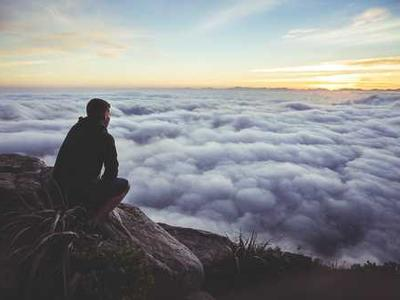
\includegraphics[height=0.5\textheight]{Images/image1.jpg}
    \end{columns}
    \vspace*{1cm}

    \note{
        \begin{itemize}
        \item Here are some notes for the second slide.
        \item These notes will appear on the second screen.
        \end{itemize}
    }

\end{frame}


% --- Slide 3: Text and Two Images ---
\begin{frame}[shrink]{Text and Two Images Slide}
    Here is some more text with two images.
    \begin{itemize}
        \item This is the second level of the notes.
        \item You can add more levels if needed.
    \end{itemize}

    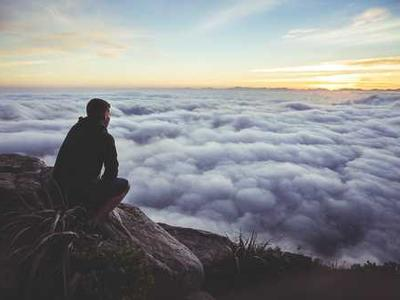
\includegraphics[width=0.48\textwidth]{Images/image1.jpg}
    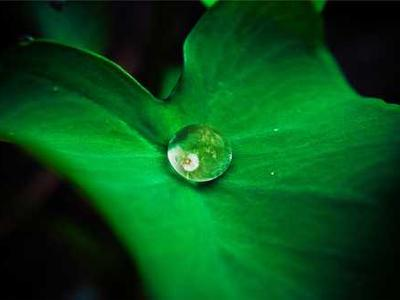
\includegraphics[width=0.48\textwidth]{Images/image2.jpg}

    \vspace*{1cm}

    \note{
        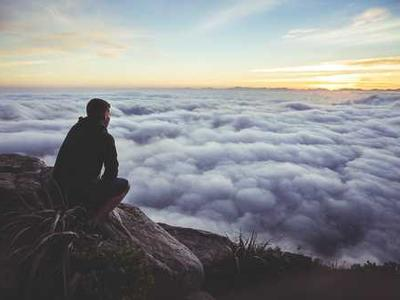
\includegraphics[width=0.5\textwidth]{Images/image1.jpg}
        \begin{itemize}
            \item You can also add images to the notes.
            \item If you ever feel you need that.
        \end{itemize}
    }

\end{frame}


% --- Slide 4: Three Images, No Text ---
{
    \newcommand{\imgheight}{0.35\textheight} % Define a variable for height
    \begin{frame}{Images Only}
        \centering
        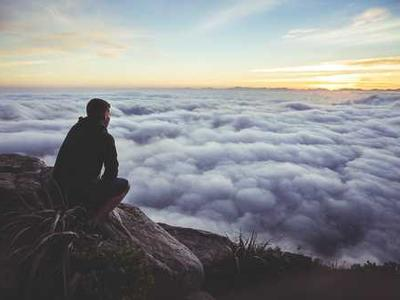
\includegraphics[width=0.48\textwidth, height=\imgheight, keepaspectratio]{Images/image1.jpg}
        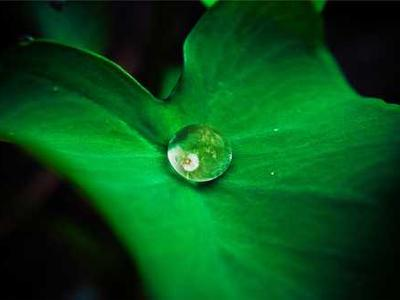
\includegraphics[width=0.48\textwidth, height=\imgheight, keepaspectratio]{Images/image2.jpg}
        
\includegraphics[width=0.48\textwidth, height=\imgheight, keepaspectratio]{Images/image3.jpg}
    \end{frame}
}

% --- Slide 5: QR Code ---
{
    % Set background color
    \setbeamertemplate{background canvas}{%
    \begin{tikzpicture}[remember picture, overlay]
      \fill[customtext]([xshift=5pt,yshift=-5pt]current page.north west) rectangle
      ([xshift=-5pt,yshift=1cm]current page.south east);
    \end{tikzpicture}%
    }
    \begin{frame}
        \color{white} % Ensures all text in the frame is white

        \begin{columns}
            \column{0.3\textwidth}
            
\includegraphics[width=4.5cm]{Logos/qr_code_innraum_eu.png}
            \column{0.5\textwidth}
            \centering
            {\Large\markhighlight{INNOVATION VERBINDET}}\\[0.5cm]
            {\Huge INNRAUM.EU}\\[1.0cm]
        \end{columns}
        \vspace*{1cm}
    \end{frame}
}

\end{document}
